\documentclass{article}
% Chinese
% \documentclass[UTF8, nofonts, mathptmx, 12pt, onecolumn]{article}
% \usepackage{xeCJK}
% \setCJKmainfont{SimSun}
\usepackage{amsmath}
\usepackage{amsfonts}
\usepackage{amssymb}
\usepackage{wasysym}
% \usepackage{ctex}
\usepackage{graphicx}
\usepackage{float}
\usepackage{geometry}
\geometry{a4paper,scale=0.8}
\usepackage{caption}
\usepackage{subcaption}
% \newcommand{\oiint}{\mathop{{\int\!\!\!\!\!\int}\mkern-21mu \bigcirc} {}}
\newcommand*{\dif}{\mathop{}\!\mathrm{d}}
\newcommand*{\md}{\mathop{}\!\mathrm{d}}
\newcommand*{\me}{\mathrm{e}}

\usepackage{parskip}
\setlength{\parindent}{0cm}

\usepackage{bm}
\let\Oldmathbf\mathbf
\renewcommand{\mathbf}[1]{\boldsymbol{\Oldmathbf{#1}}}
\let\eqnarray\align

\author{Xiping Hu}
\usepackage{authblk}
\author{Xiping Hu}
\affil{http://thehxp.tech/}
\title{Homework for Analogue Electronics}

\begin{document}
\maketitle

\begin{figure}[H]
  \centering
  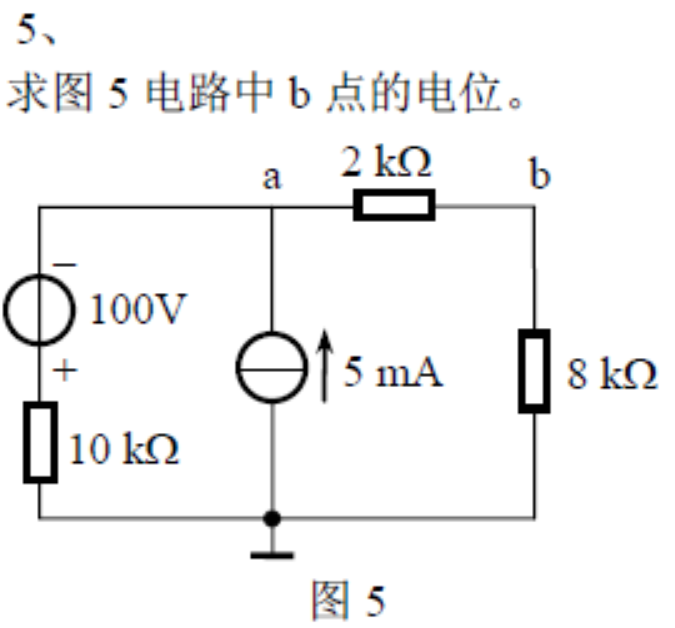
\includegraphics[width=\linewidth]{figures/5}
  \label{fig:}
\end{figure}

\paragraph{Solution}

We separate the whole circuit into these two sub-circuits, as the picture below shows.

\begin{figure}[H]
  \centering
  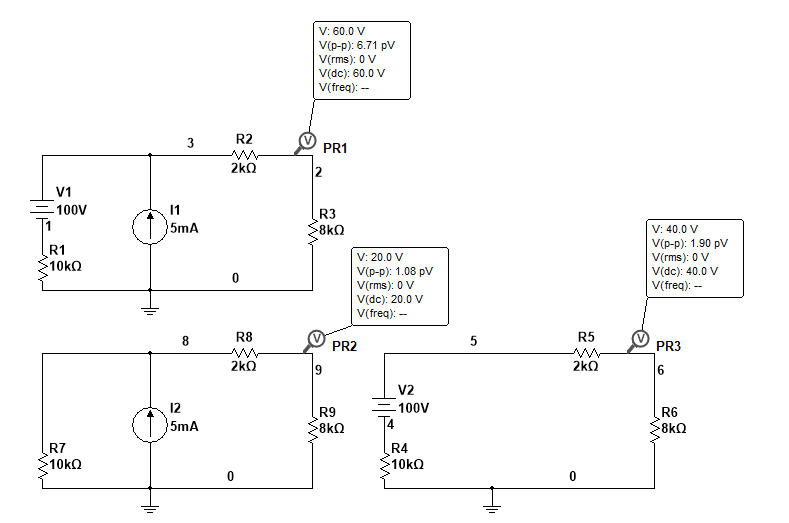
\includegraphics[width=\linewidth]{figures/9}
  \label{fig:}
\end{figure}

For the circuit on the bottom left position, we write
\begin{equation*}
  \begin{aligned}
    I = 5 \  \mathrm{mA} \times \dfrac{10 \  \mathrm{k\Omega}}{2 \  \mathrm{k\Omega} + 8 \  \mathrm{k\Omega} + 10 \  \mathrm{k\Omega}} = 2.5 \  \mathrm{mA}
  \end{aligned}
\end{equation*}
\begin{equation*}
  \begin{aligned}
    U = I R = 2.5 \  \mathrm{mA} \times 8 \  \mathrm{k\Omega} = 20 \  \mathrm{V}
  \end{aligned}
\end{equation*}
For the circuit on the bottom right
\begin{equation*}
  \begin{aligned}
    I = \dfrac{100 \  \mathrm{V}}{10 \  \mathrm{k\Omega} + 2 \  \mathrm{k\Omega} + 8 \  \mathrm{k\Omega}} = 5 \  \mathrm{mA} 
  \end{aligned}
\end{equation*}
\begin{equation*}
  \begin{aligned}
    U = 5 \  \mathrm{mA} \times 8 \  \mathrm{k\Omega} = 40 \  \mathrm{V}
  \end{aligned}
\end{equation*}
So, as for the original circuit
\begin{equation*}
  \begin{aligned}
    U_b = 20 \  \mathrm{V} + 40 \  \mathrm{V} = 60 \  \mathrm{V}
  \end{aligned}
\end{equation*}





\end{document}